\documentclass{scrreprt}
\usepackage{graphicx}
\usepackage{listings}
\usepackage{underscore}
\usepackage[bookmarks=true]{hyperref}
\usepackage[utf8]{inputenc}
\usepackage[english]{babel}
\usepackage{subfigure}
\usepackage{hyperref}
\usepackage[table,xcdraw]{xcolor}
\usepackage[most]{tcolorbox}
\setlength{\footskip}{140pt}
\graphicspath{ {images/} } 
\hypersetup{
    bookmarks=false,    % show bookmarks bar?
    pdftitle={Software Requirement Specification},    % title
    pdfauthor={Matthew Berger},                     % author
    pdfsubject={TeX and LaTeX},                        % subject of the document
    pdfkeywords={TeX, LaTeX, graphics, images}, % list of keywords
    colorlinks=true,       % false: boxed links; true: colored links
    linkcolor=blue,       % color of internal links
    citecolor=black,       % color of links to bibliography
    filecolor=black,        % color of file links
    urlcolor=purple,        % color of external links
    linktoc=page            % only page is linked
}%
\def\myversion{2.0 }
\date{}
%\title
\usepackage{xcolor,colortbl}
\newcommand{\mc}[2]{\multicolumn{#1}{c}{#2}}
\definecolor{LightGray}{gray}{0.95}
\definecolor{Gray}{gray}{0.85}
\definecolor{LightCyan}{rgb}{0.88,1,1}

\newcolumntype{a}{>{\columncolor{Gray}}p{0.3\linewidth}}
\newcolumntype{b}{>{\columncolor{white}}p{0.7\linewidth}}
\newcolumntype{d}{>{\columncolor{LightGray}}p{0.3\linewidth}}
\newcolumntype{e}{>{\columncolor{white}}p{0.6\linewidth}}
\newcolumntype{f}{>{\columncolor{LightGray}}p{0.2\linewidth}}
\newcolumntype{g}{>{\columncolor{Gray}}p{0.2\linewidth}}
\newcolumntype{h}{>{\columncolor{white}}p{0.8\linewidth}}
% A special box for this
\newtcolorbox{highlightbox}[1][]{colback=yellow,enhanced jigsaw, sharp corners,box align=center,boxrule=0pt,boxsep=0pt,#1}

\begin{document}

\begin{flushright}
    \rule{16cm}{5pt}\vskip1cm
    \begin{bfseries}
        \Huge{SOFTWARE DESIGN DOCUMENT SPECIFICATION}\\
        \vspace{1.6cm}
        for\\
        \vspace{1.6cm}
        $NAVATAR$\\
        \vspace{1.6cm}
        \LARGE{Version \myversion approved}\\
        \vspace{1.6cm}
        Prepared by Matthew Berger, Liam Gomez, and Connor Parkinson\\ 
        \vspace{1.6cm}
        Advised by Professor Eelke of the\\UNR CSE Department\\
        \vspace{1.6cm}
        \today\\
    \end{bfseries}
\end{flushright}

\tableofcontents

\chapter*{Revision History}

\begin{center}
    \begin{tabular}{|c|c|c|c|}
        \hline
	    Name & Date & Reason For Changes & Version\\
        \hline
	    Matthew Berger & 11/29/16 & Created document & 1.0.0\\
        \hline
        Matthew Berger & 4/19/17 & Created document revision & 2.0.0\\
        \hline
    \end{tabular}
\end{center}

\chapter{Overview}

	\section{Abstract}
Navatar is an indoor navigation system for visually impaired students. Unlike existing systems that rely on expensive equipment, Navatar only requires an Android smartphone. The phone’s GPS and accelerometer are used to approximate a user's location and movements and the phone’s speaker is used to provide auditory directions to rooms within a building. Buildings on University campuses often have the GIS maps and the design required for Navatar’s accelerometer based localization, which is why students are the intended audience for the project. With the application’s open source status and modular design, crowdsourcing efforts can be used to integrate maps for buildings on any campus.\begin{highlightbox}The application's improvements are nearing completion and Team 6 has worked on a variety of new features alongside other open source contributors. Currently, the features completed are as follows: Geo-Fencing, Gesture Detection, Optimization for Google Talkback, Route History, and Route Reversal. Geo-Fencing is determining the building a user might be in based on their current GPS coordinates and some mathematics. The gesture detection system allows the user to operate the application during navigation so that custom actions may be added. Google Talkback is used to control the application when a navigation is not currently in progress, and the application is now optimized for the easiest possible use with Google Talkback so that blind users who are familiar with navigating apps via Talkback will have a seamless experience. Route history allows users to select routes from paste navigations. Route reversal allows users to take a route that they have already taken, except in reverse. This is effective for navigating back to a starting location after a class ends, etc. In addition to this, code cleanup was performed and any piece of the codebase that was touched was improved as a rule.\end{highlightbox}
\pagebreak
	\section{Introduction}
The main goals and objectives of this project are to help blind people navigate indoor environments using a mobile phone and open source software which allows for a very low overall cost. Most people already have a cell phone, and mobile phones have a wide array of sensors available for environmental information. Accessibility is a major issue for many students with disabilities, and the technology necessary to ease the burden of some tasks that can be needlessly complicated is available and waiting to be utilized. Currently, there is no free and open source software capable of gathering environmental information and assisting students with indoor navigation for an entire college campus.
    The high level requirements of this software include being simple to use, low-cost, scalable, maintainable, and efficient in its assistance to blind users. The intended audience of this project, as stated, is blind students and partially blind students. Existing and familiar environments will be conquered through the use of landmarks and bookmarks. A bookmark in this case would be a landmark that the user sets manually, that gets stored specifically for that user. The reason behind this is that many partially-sighted and blind users remember details that sighted people may not utilize or need, such as a metal strip on the floor, that help them remember where they are in an indoor setting relative to where they want to go.
    The project itself currently exists as a repository on GitHub that contains a mobile android app. The members Team 6 all currently have a fork and are working on learning the code base to facilitate the development of new features. The future of this software depends greatly on what we are capable of achieving in the time-frame provided, but we plan on implementing many features. The first planned enhancement is the implementation of geofencing to determine what building the user is in. Possible future enhancements include the ability for users to declare and input their own landmarks, third party device integration to improve usability and accuracy (i.e. smart watches, Bluetooth earpieces), using additional environment information such as wifi SSIDs, making the app more scalable, improving map conversion and creation, user profile learning, stride detection, and gesture-based UI/UX improvements.
\chapter{Design}
	\section{Navatar Software Architecture}
		This can be found in an attachment with this document, since the diagram is rather large.
		\includegraphics[width=\textwidth,height=0.4\textheight]{navatar.jpg}
	\pagebreak
	\section{Detailed Design}
		\subsection{Manual and Geofence Building Selection}
			\includegraphics[width=\textwidth]{design1.jpg}
		\pagebreak	
		\subsection{Geofencing}
			\includegraphics[width=\textwidth,height=0.8\textheight,keepaspectratio]{design2.png}
		\subsection{Navigation Instructions and Adding Landmarks}
			\includegraphics[width=\textwidth]{design3.png}
		\subsection{Navigation Instructions and Adding Landmarks}
			\includegraphics[width=\textwidth]{design3.png}
	\section{Initial Hardware Design}
	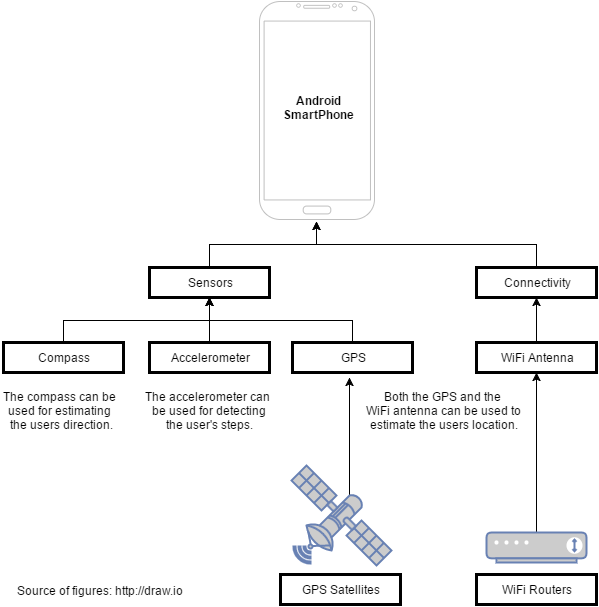
\includegraphics[width=\textwidth]{hwdesign.png}
\pagebreak
\begin{figure}[ht!]
\chapter{Snapshots}
\section{User Interface Design}
These screenshots demonstrate intended user interface design of the software. The software is meant for blind users however, so the UI demonstrated here would be navigated with audio cues or swiping gestures in the final application.
     \begin{center}
%
        \subfigure[Starting Location Selection]{%
            \label{fig:first}
            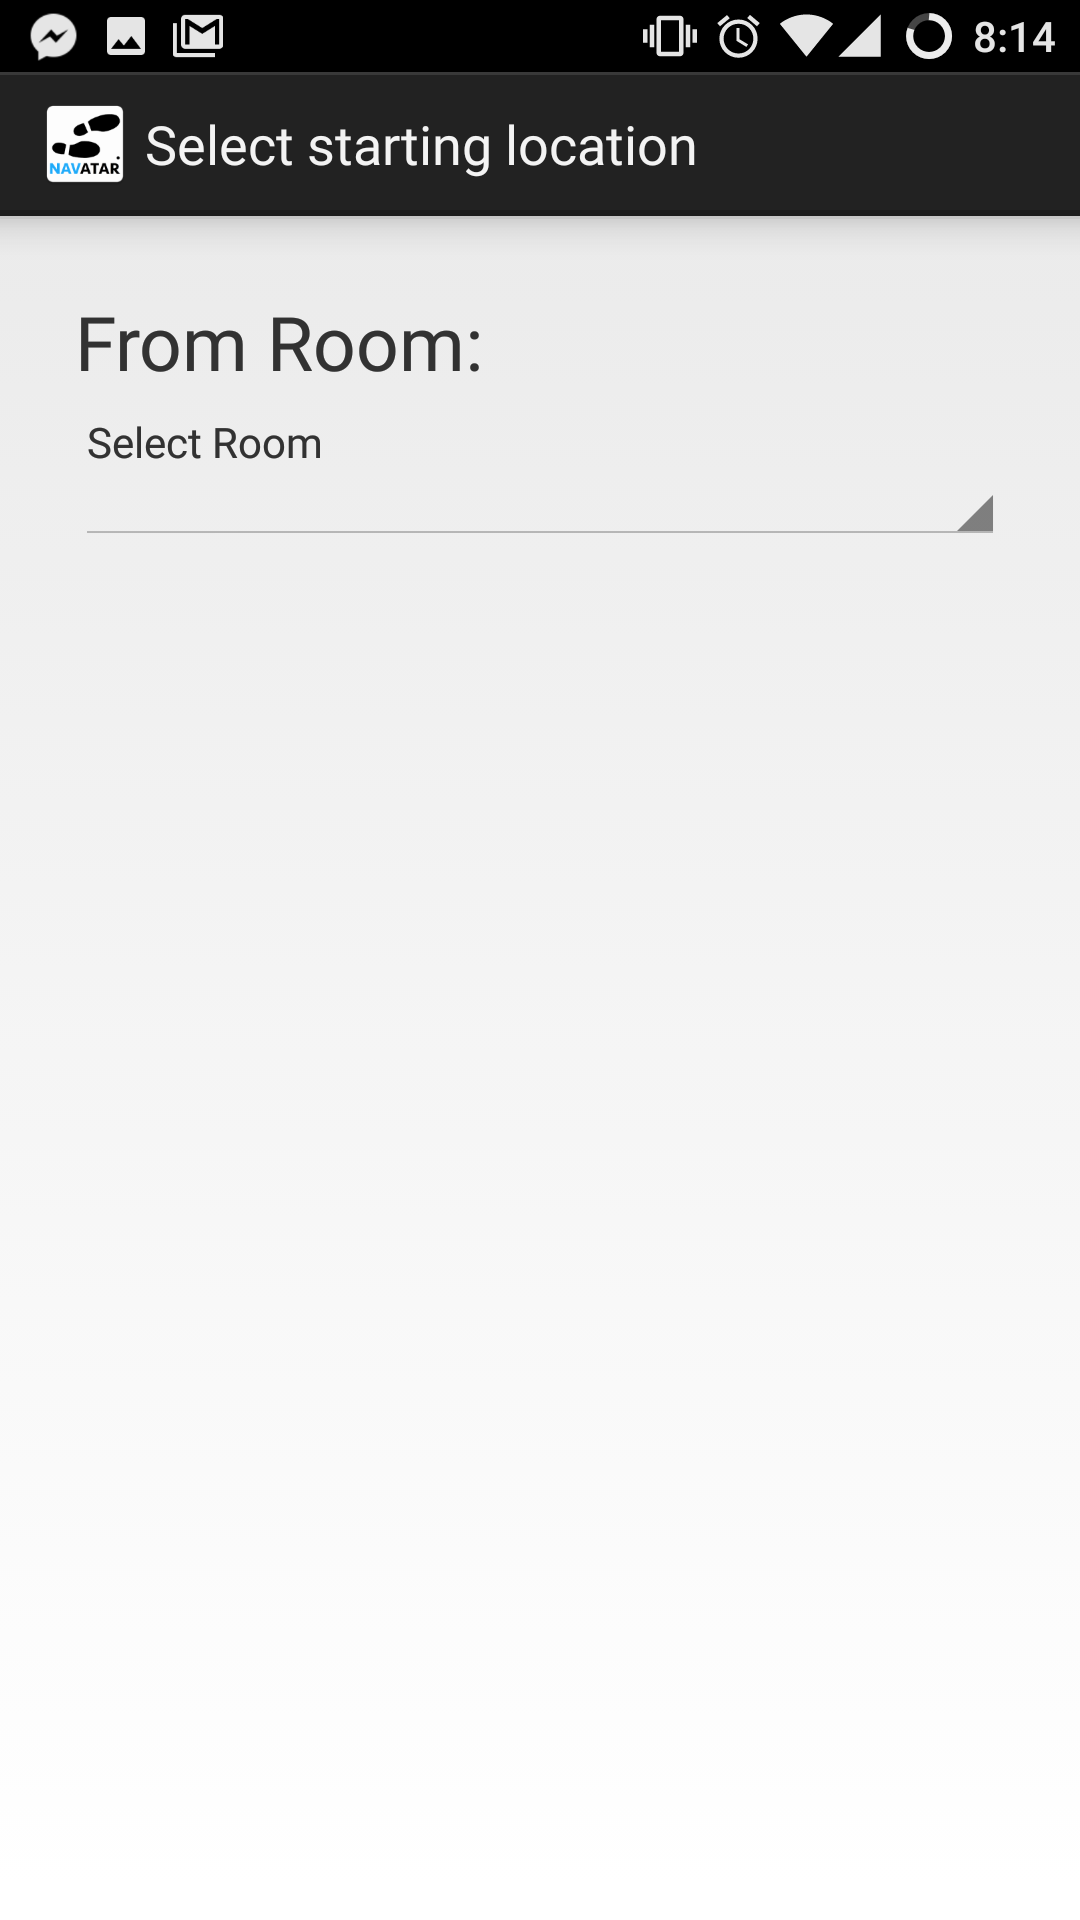
\includegraphics[width=0.3\textwidth]{1.png}
        }%
        \subfigure[Destination Selection]{%
           \label{fig:second}
           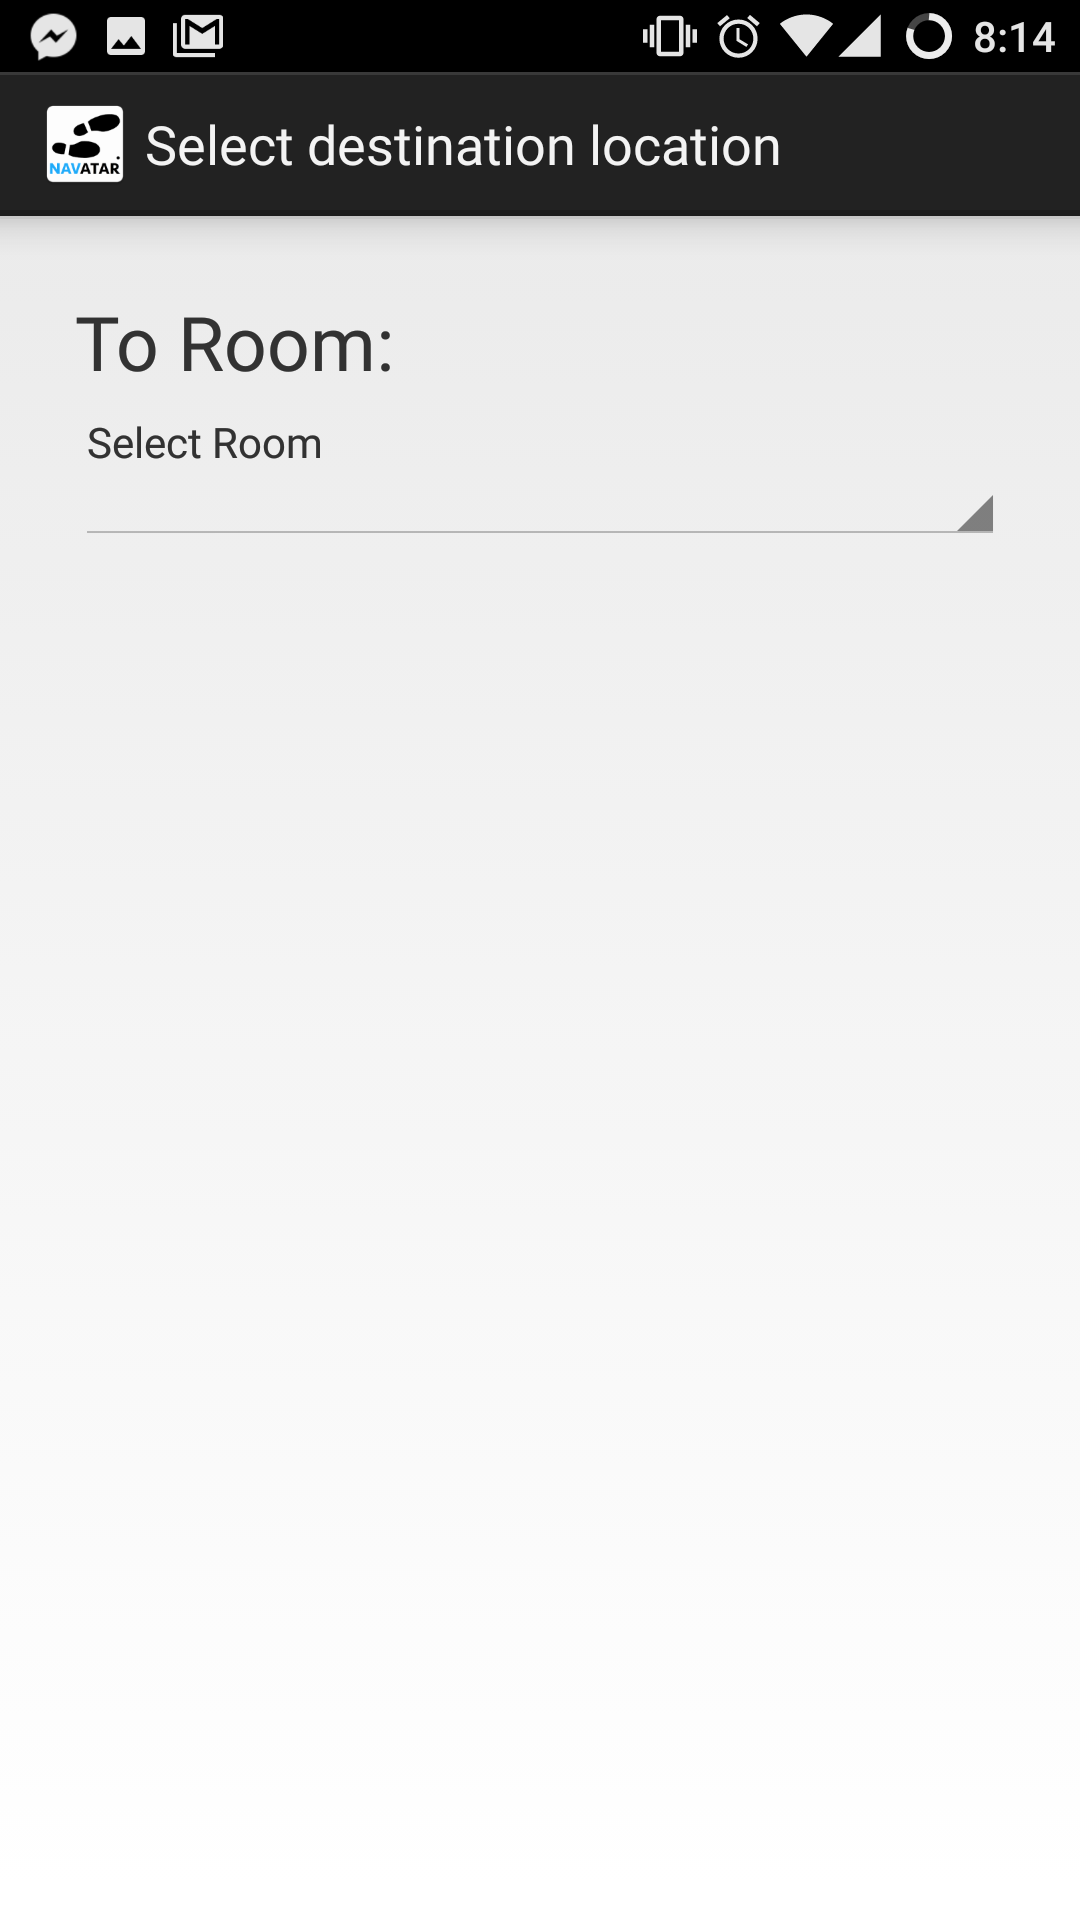
\includegraphics[width=0.3\textwidth]{2.png}
        } %  ------- End of the first row ----------------------%
        \subfigure[Arrival Screen]{%
            \label{fig:third}
            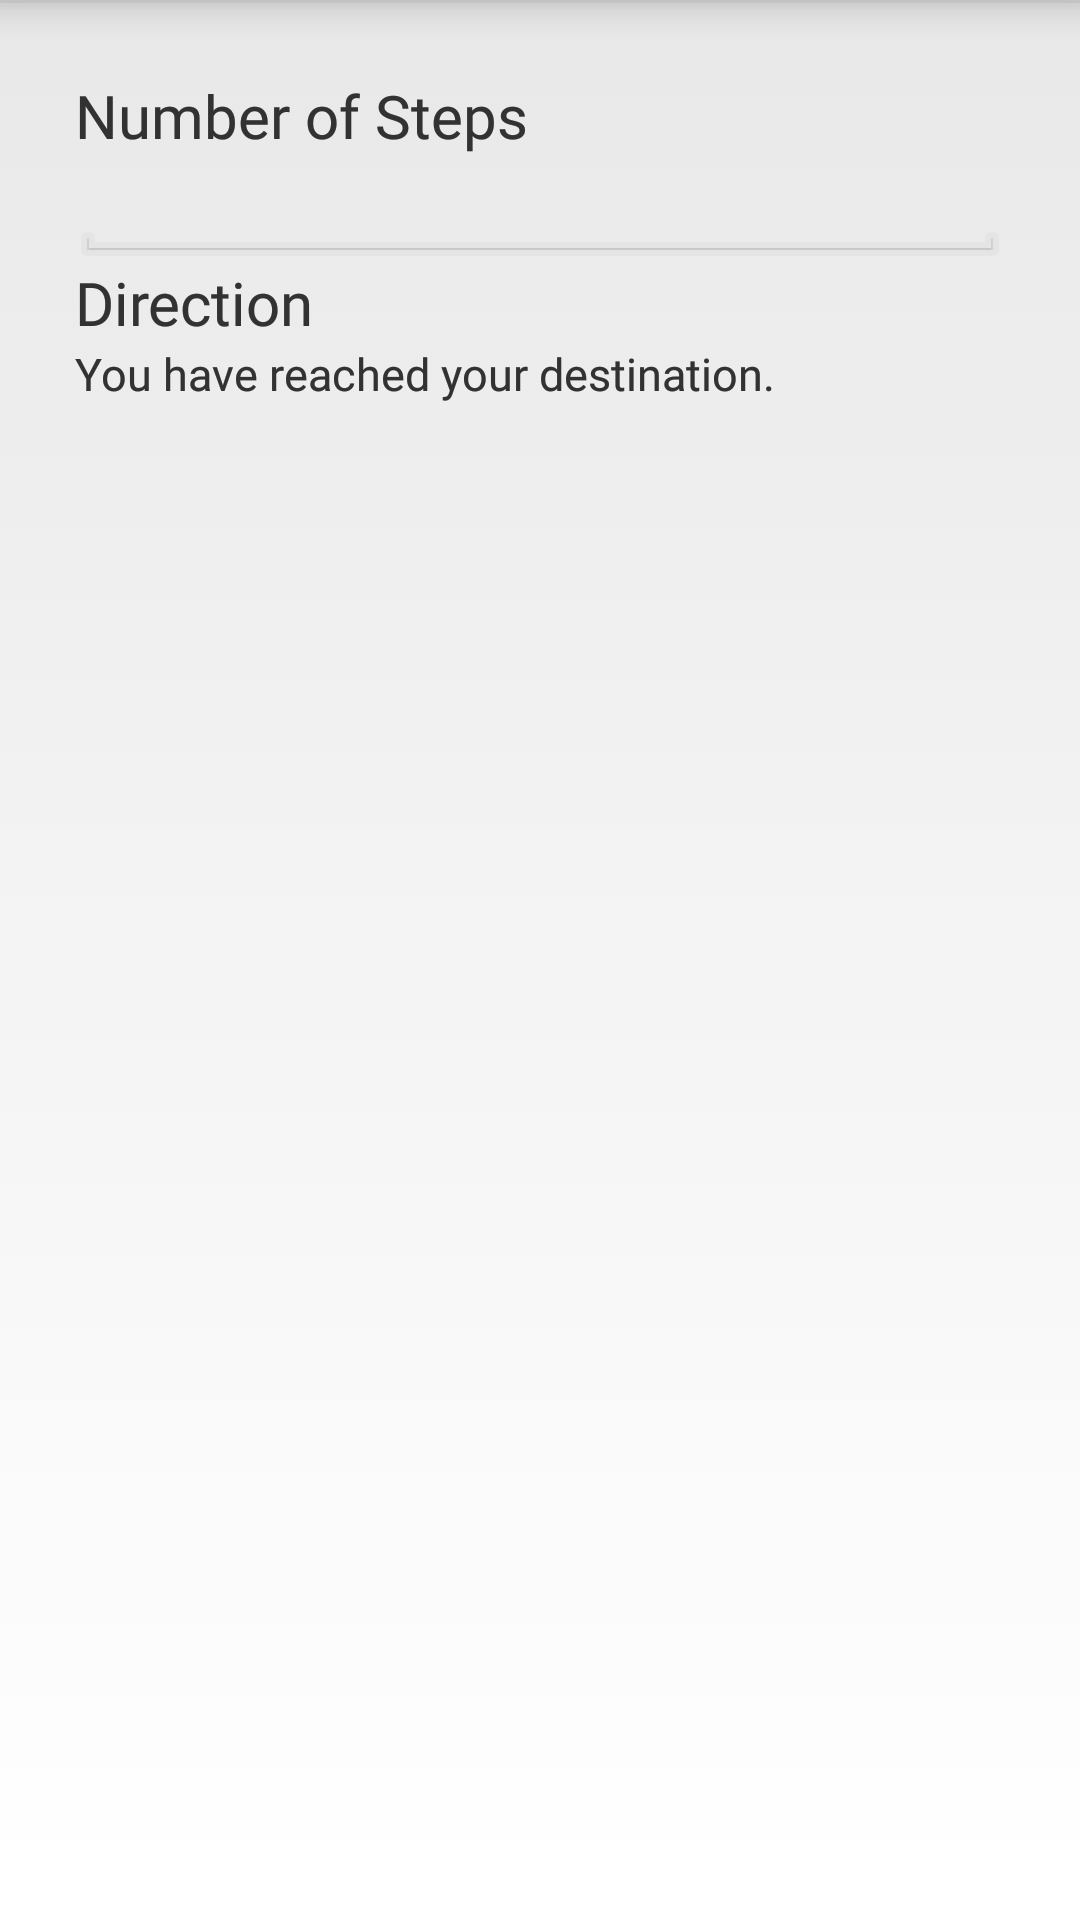
\includegraphics[width=0.3\textwidth]{3.png}
        }\\%
        \subfigure[Adding Landmarks]{%
            \label{fig:fourth}
            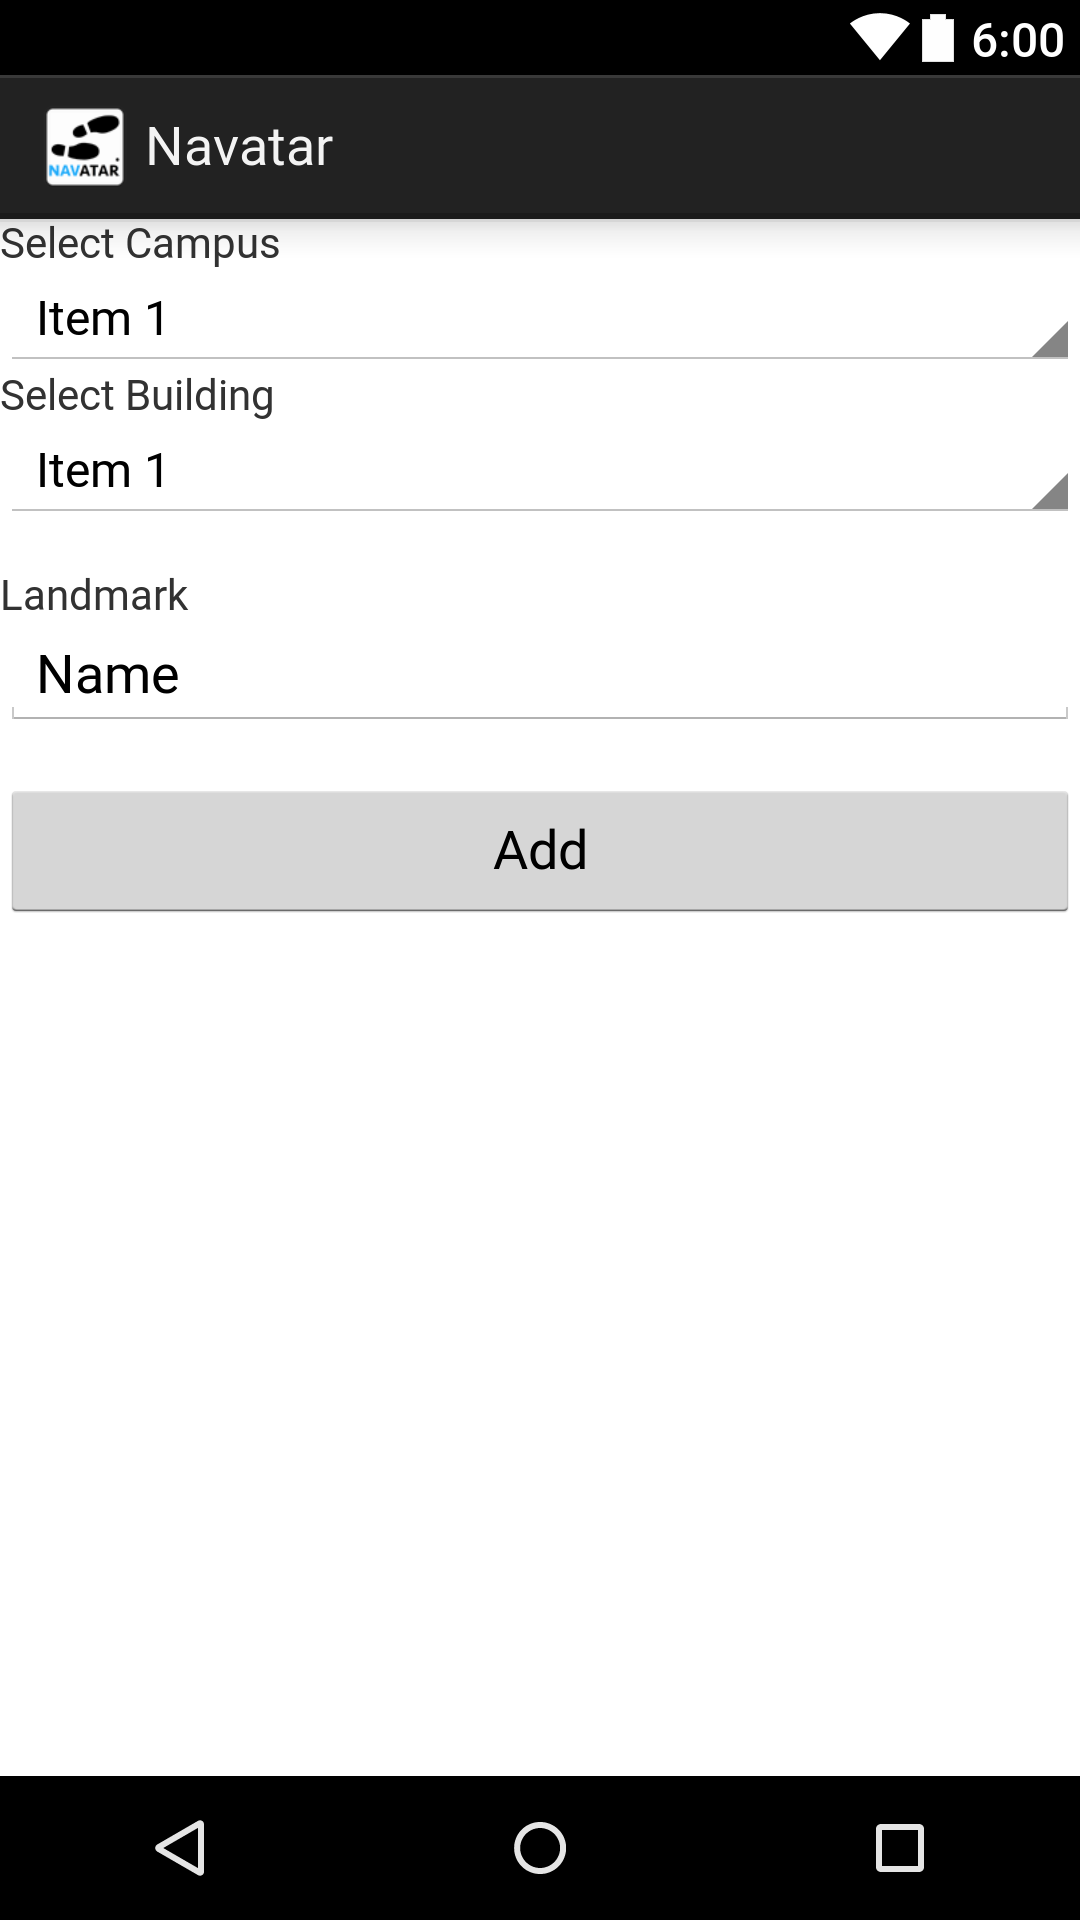
\includegraphics[width=0.3\textwidth]{4.png}
        }%
        \subfigure[Building Detection]{%
           \label{fig:fifth}
           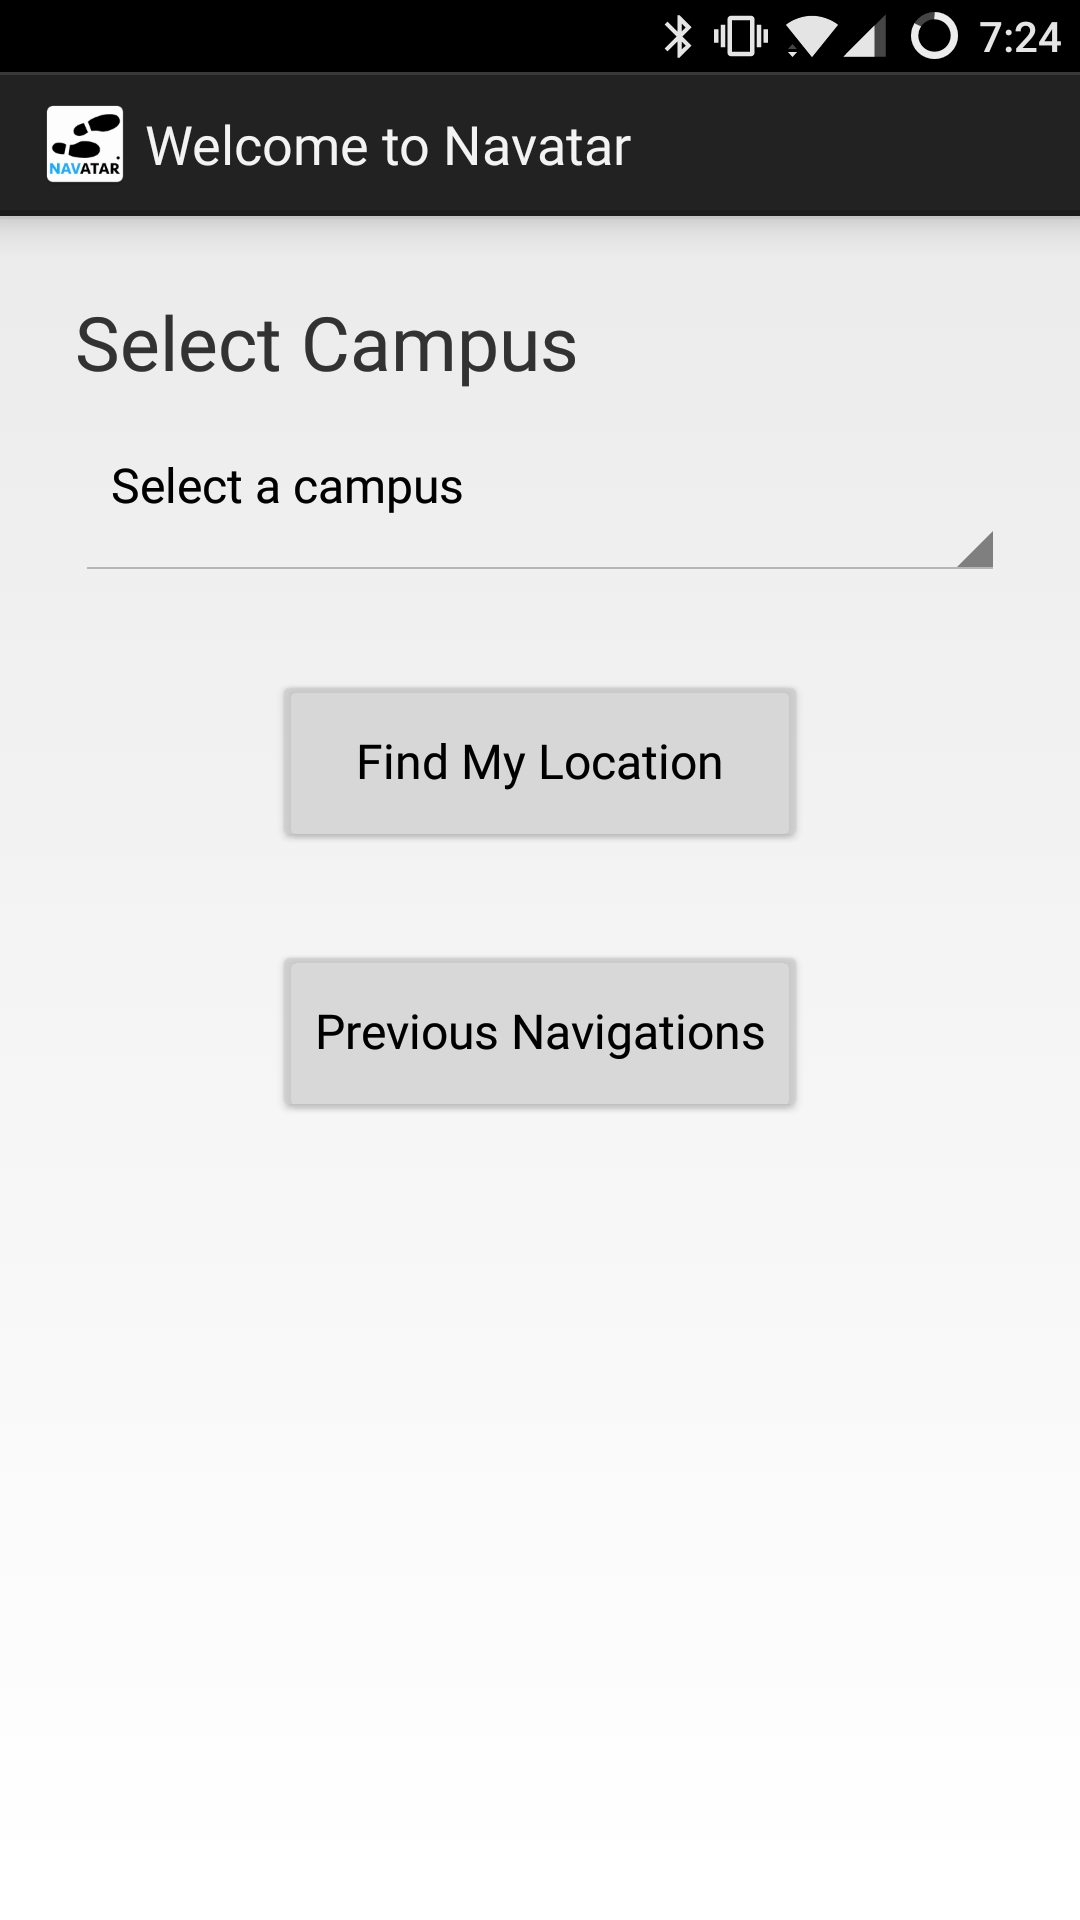
\includegraphics[width=0.3\textwidth]{5.png}
        } 
%
    \end{center}
    \caption{%
        User Interface Screenshots
     }%
   \label{fig:subfigures}
\end{figure}

\begin{figure}[ht!]

\section{Layout}
     \begin{center}
%
        \subfigure[Home Screen]{%
            \label{fig:first}
            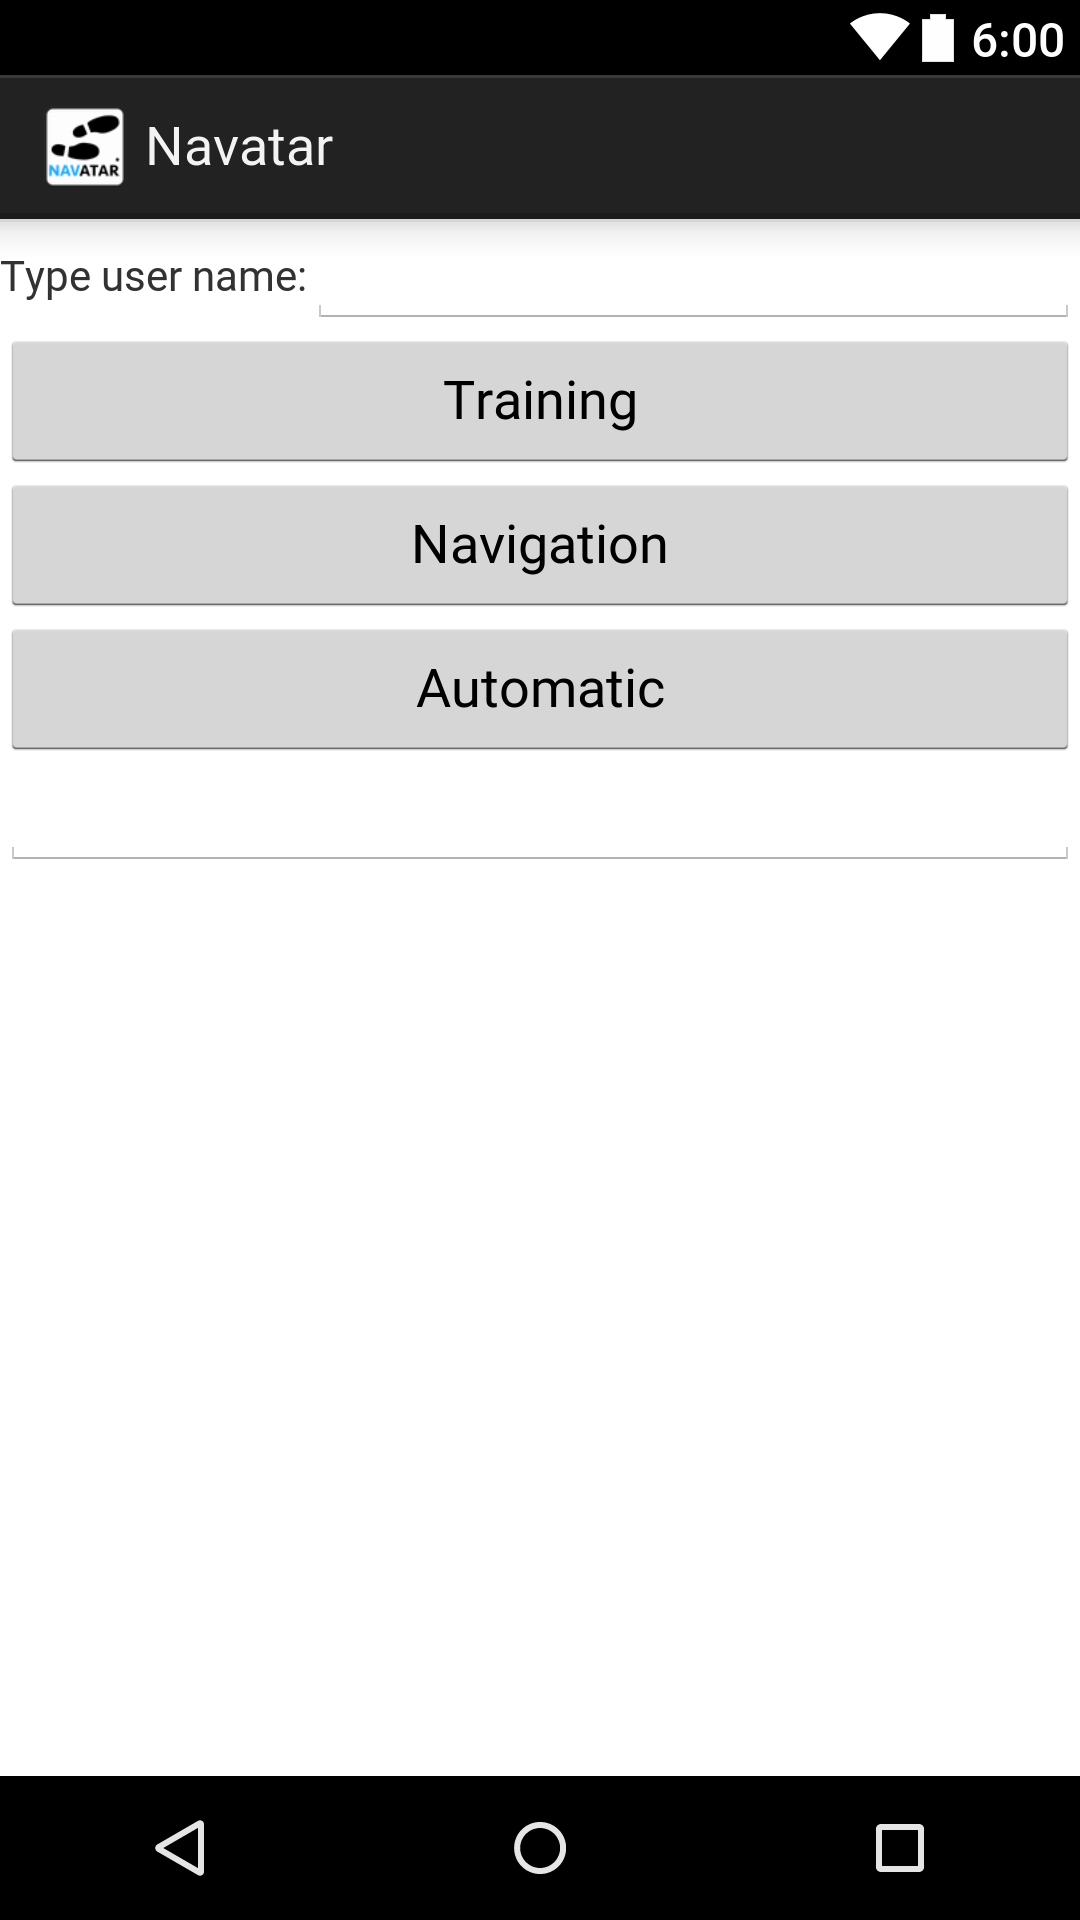
\includegraphics[width=0.3\textwidth]{11.png}
        }%
        \subfigure[Navigation Screen]{%
           \label{fig:second}
           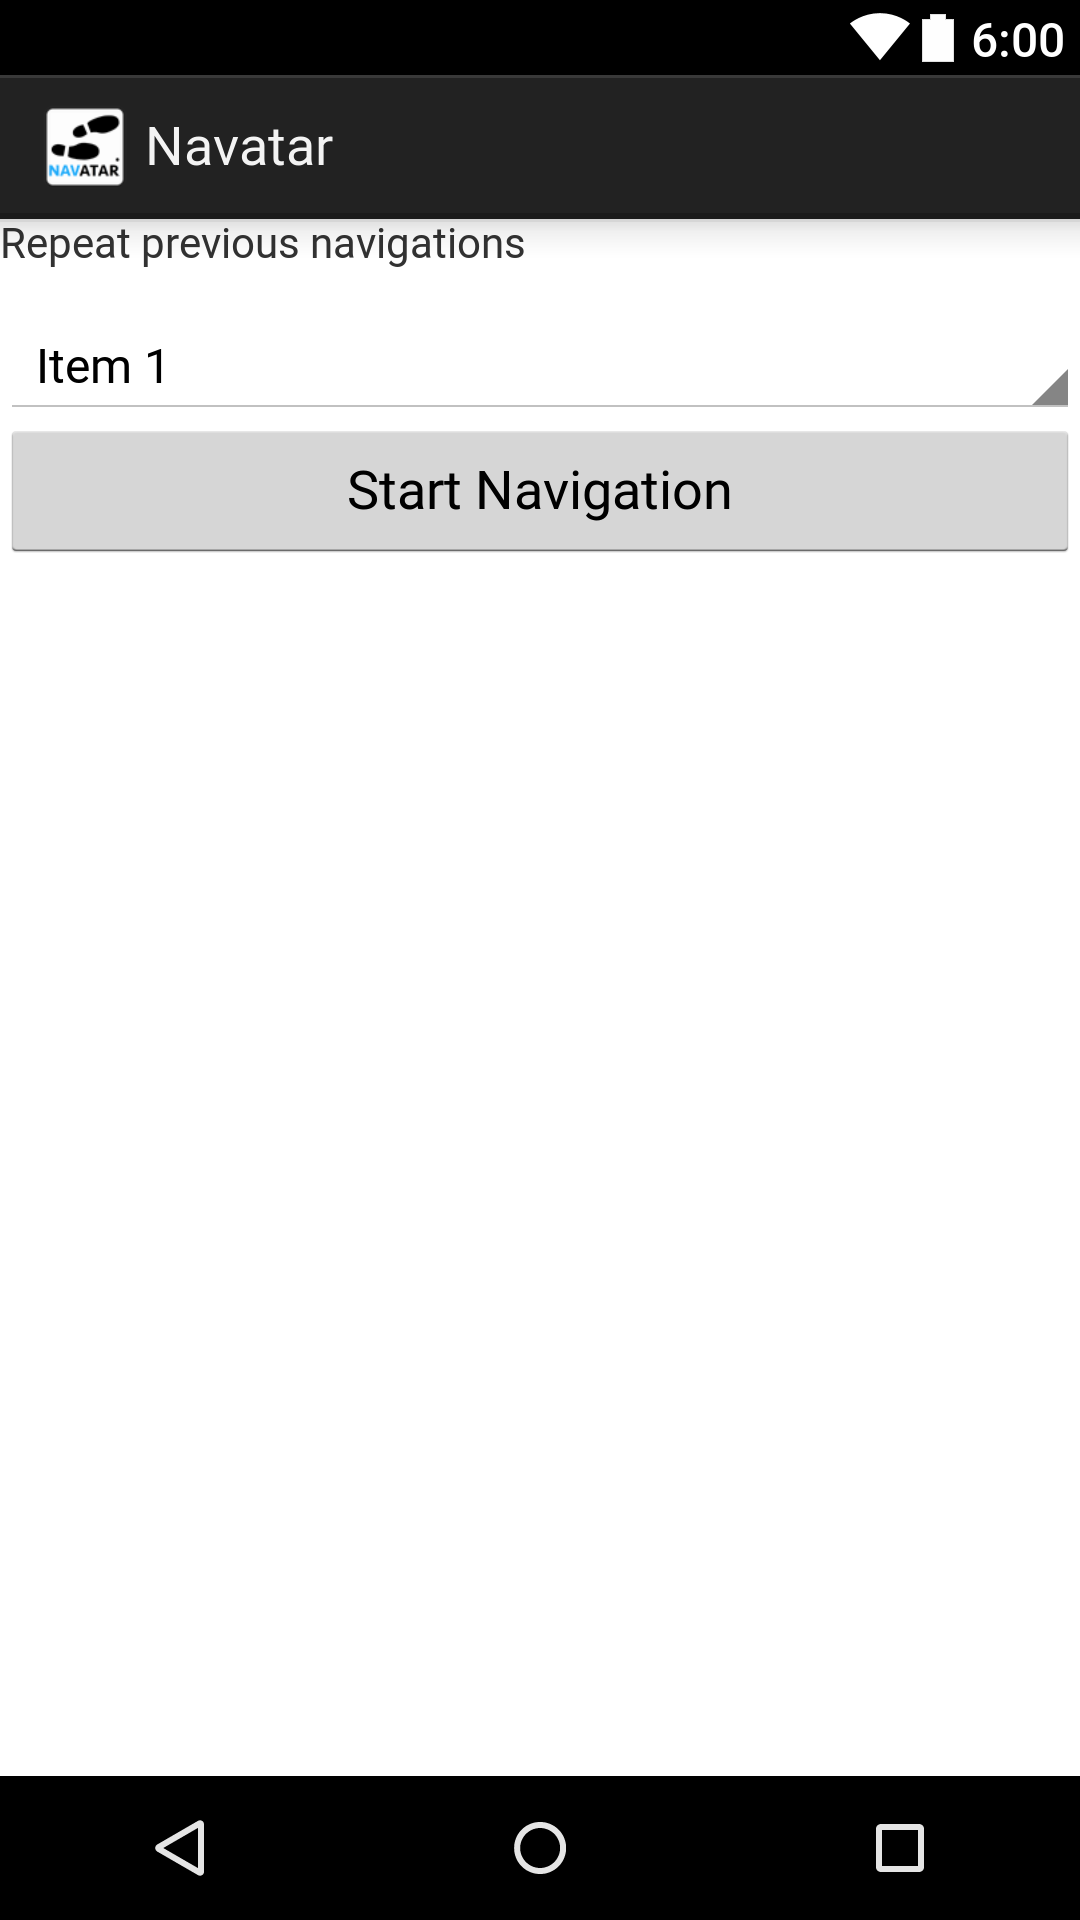
\includegraphics[width=0.3\textwidth]{12.png}
        } %  ------- End of the first row ----------------------%
        \subfigure[User Profile Settings]{%
            \label{fig:third}
            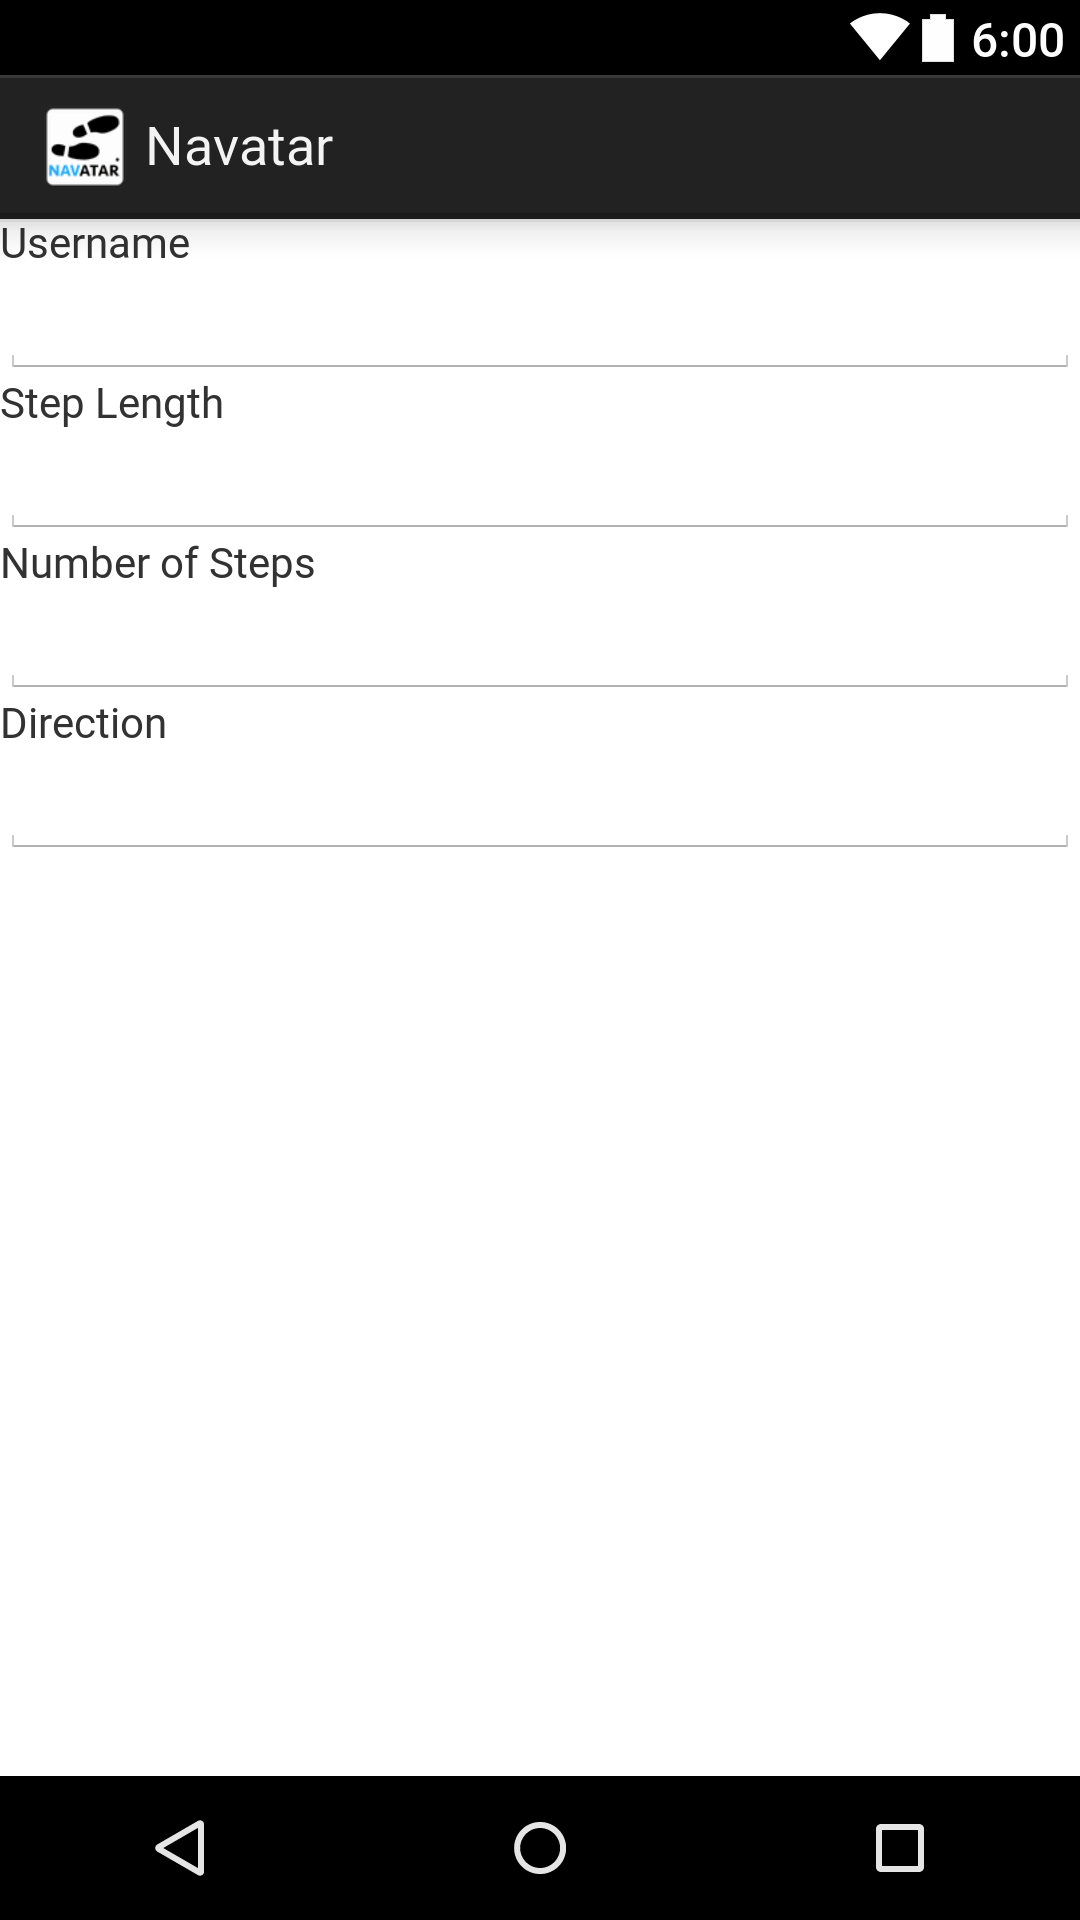
\includegraphics[width=0.3\textwidth]{13.png}
        }\\%
        \subfigure[Application Launch Screen]{%
            \label{fig:fourth}
            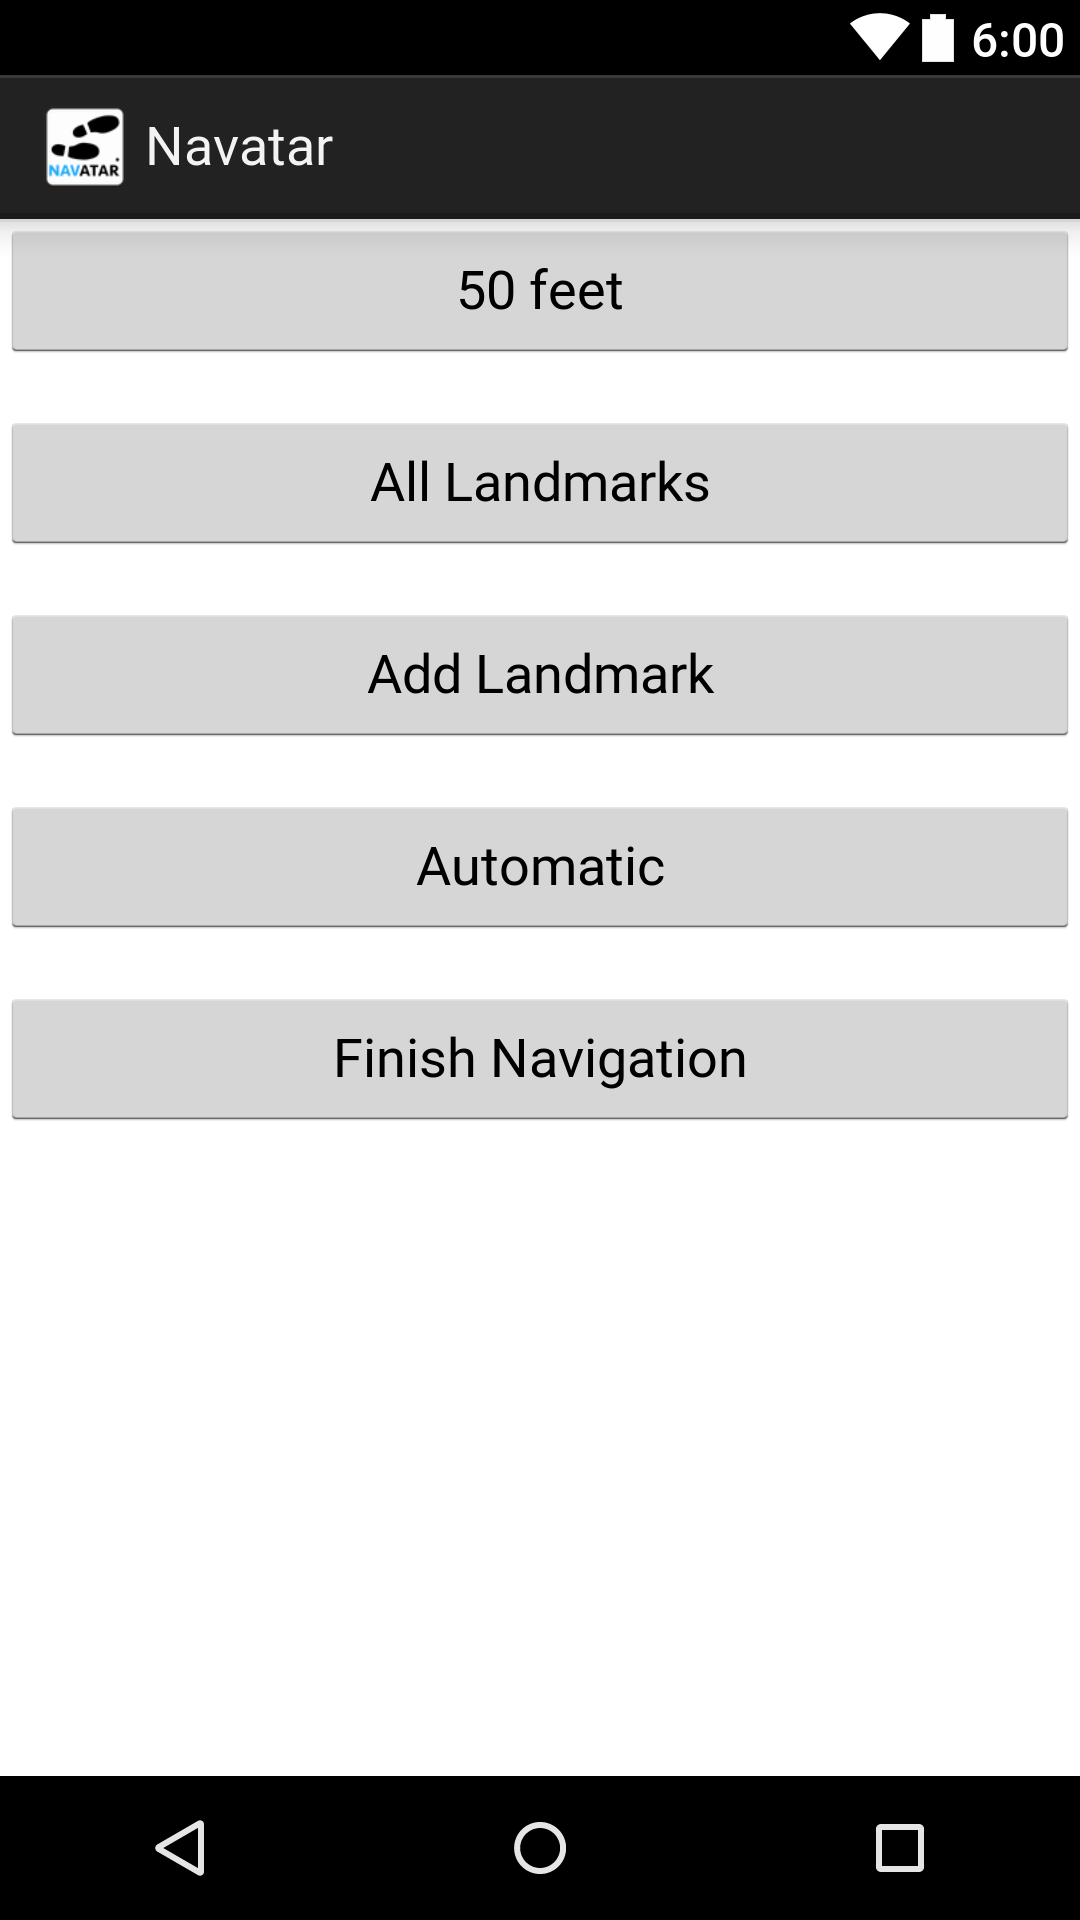
\includegraphics[width=0.3\textwidth]{14.png}
        }%\\
        \subfigure[Route History Screen]{%
            \label{fig:fifth}
            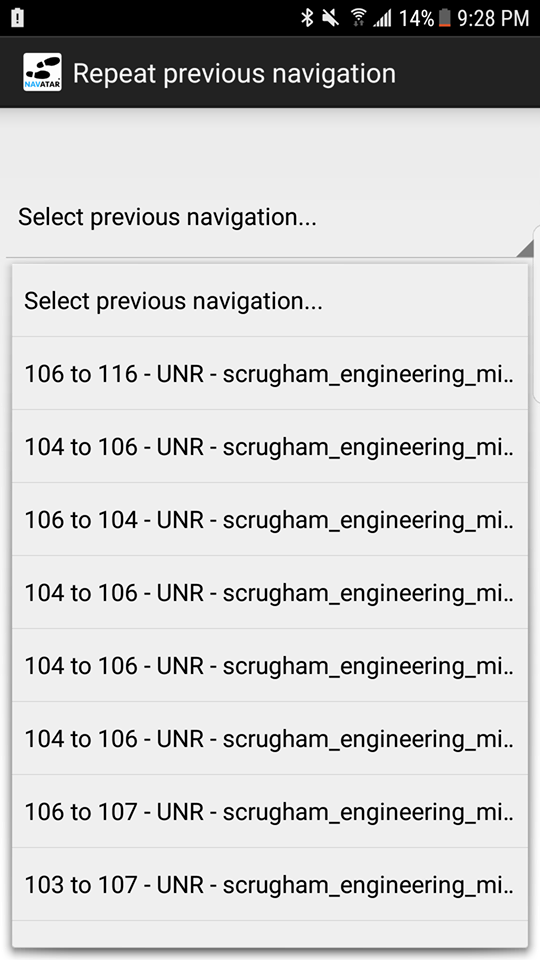
\includegraphics[width=0.3\textwidth]{routes.png}
        }%
        
        \begin{highlightbox}
        	Update: Route history screenshot added.
        \end{highlightbox}
%
    \end{center}
    \caption{%
        Layout Screenshots
     }%
   \label{fig:subfigures}
\end{figure}
	
\chapter{References}

\section{Feasibility of Interactive Localization}
Ilias Apostolopoulos, Navid Fallah, Eelke Folmer, Kostas Bekris. Feasibility of Interactive Localization and Navigation of People with Visual Impairments, Proceedings of 11th Intelligent Autonomous Systems Conference, Pages 22-32, Ottawa, Ontario, August 2010.\\
 
 \textbf{Summary:}
Investigates various solutions to the problem of indoor navigation for the visually impaired. Describes the issues that make indoor localization systems difficult to implement, and weighs the pros and cons of solutions that are currently available. These solutions include using RFID tags, cameras, or range finders to provide locational information. These solutions are quite expensive due to high installation and equipment costs. The article proposes the use of common smartphone sensors in combination with user interaction and user provided landmarks to provide navigational information to the user. Provides technical specifications for estimating a user’s location.
 
\section{Results from Initial User Experiments of Navatar}
Ilias Apostolopoulos, Navid Fallah, Eelke Folmer, Kostas Bekris, Integrated Online Localization and Navigation for People with Visual Impairments using Smart Phones, IEEE International Conference on Robotics and Automation (ICRA), Pages 1322 -1329, Minnesota, MN, May, 2012.\\

\textbf{Summary:}
Discusses the results from initial user experiments with the Navatar prototype, providing detailed statistical data and analysis. In depth description of Navatar’s path planning algorithm and accuracy. Shares some of the user’s experiences and feedback. The user’s experiences were all positive, saying that directions were clear and that the application did have potential to prevent the user from getting lost in new buildings. The users did suggest some possible improvements, including accuracy improvements, saving and repeating directions, and making the application hands free.
\pagebreak
\section{Navatar’s Localization Architecture}
 Ilias Apostolopoulos, Navid Fallah, Eelke Folmer, Kostas Bekris. Integrated Online Localization and Navigation for People with Visual Impairments using Smart Phones, ACM Transactions on Interactive Intelligent Systems 3:4, Pages 1-25.\\

\textbf{Summary:}
More in depth descriptions of Navatar’s localization architecture, giving the actual algorithms used for sampling, as well as the transition and observation models. Shows how the K-Means algorithm can be used to adapt Navatar’s localization system to the unique stride lengths of a given user. Discusses potential limitations due to the computational ability of smartphones, proposes an offline training process using better hardware to solve this problem. Briefly describes Navatar’s user interface design and the UI’s accessibility to those with visual impairments.

\section{Indoor Navigation System for the Blind}
Scientists design indoor navigation system for blind. (2016). Phys.org. Retrieved 8 November 2016, from http://phys.org/news/2012-05-scientists-indoor.html\\

\textbf{Summary:}
 A high level overview of indoor localization systems, describing how Navatar uses a combination of GIS maps and readily available smartphone sensors to help visually impaired users navigate buildings. Contains some interview questions answered by Eelke Folmer about Navatar, and the potential benefits it could have. Folmer discusses some of the obstacles that had to be overcome in the development of Navatar, as well as his motivation for the creation of Navatar.


\chapter{Contributions}
\begin{highlightbox}These contributions took place over the course of the Fall 2016 semester through to the end of the Spring 2017 semester at UNR. Because the features were large and self-contained, all of the time utilized was spent ensuring the necessary functionality was implement and that the desired code cleanup was performed.\end{highlightbox}
	\section{Matthew Berger}
		\begin{itemize}
			\item Created LaTeX document.
			\item Created cover page and table of contents.
			\item Completed software architecture diagram.
			\item \begin{highlightbox} Designed, prototyped, and implemented the gesture detection system.
			\end{highlightbox}
			\item \begin{highlightbox} Established a reproducible Vagrant development environment.
			\end{highlightbox}
		\end{itemize}
	\section{Connor Parkinson}
		\begin{itemize}
			\item Completed abstract and introduction.
			\item Created detailed design diagrams.
			\item Created initial hardware design diagram.
			
			\item \begin{highlightbox} 
			Designed, prototyped, and implemented the Geo-Fencing feature.
			\end{highlightbox}
				
			\item \begin{highlightbox}
			Handled team management and project coordination responsibilities.
			\end{highlightbox}
				
			\item \begin{highlightbox} 
			Performed optimizations for Google Talkback.
			\end{highlightbox}
		\end{itemize}
\pagebreak
	\section{Liam Gomez}
		\begin{itemize}
			\item Created mockups for the user interface changes needed for the new features.
			\item Updated the references relevant to this assignment.
			\item Added new terms to the glossary.
			\item \begin{highlightbox} 
			Designed, prototyped, and implemented the Route Reversal feature.
			\end{highlightbox}
			\item \begin{highlightbox} 
			Designed, prototyped, and implemented the Route History feature.
			\end{highlightbox}
		\end{itemize}
		
\begin{table}[ht]
\chapter{Glossary}
\centering
\def\arraystretch{1.5}%
\resizebox{0.9\textwidth}{!}{\begin{tabular}{| a | b | }
\hline
\rowcolor{LightCyan}
\mc{1}{Term}  & \mc{1}{Definition} \\
\hline
Android & An operating system for mobile devices and smartphones. Navatar currently only supports this operating system.\\
\hline
 
Android Studio & An integrated development environment (IDE) for developing mobile applications for the Android operating system.\\
 
\hline
Dead-Reckoning & A localization technique that estimates a user’s location using an old estimated location as the starting point, using various data from sensors and other environment information to improve estimations.\\
 
\hline
Direct Sensing & A localization technique that uses physical identification tags to provide the current location of a user. Direct sensing requires the installation of these tags in the environment, which can be quite expensive.\\
 
\hline
Geofencing & Using global positioning systems to create geographical boundaries around an area, useful for determining what building a user of Navatar might be entering.\\
 
\hline
Geographic Information System (GIS) & a system used to store, manipulate, and present geographical data. Geographic information system maps are used by Navatar to load the layout of a given building.\\
 
\hline
Github & A web based service that hosts Git repositories to provide source control for software development purposes.\\

\hline
Global Positioning System (GPS) & A network of navigation satellites that provides geolocation information to a GPS receiver. GPS can be unreliable in indoor environments due to signal interference from the environment.\\

\hline
Landmark-based Navigation & Navigation using physical landmarks and a physical or mental map of the environment.\\

\hline
Localization & Adaptation of a product or service to meet the needs of a given language, culture, or population.\\
 
\hline
Pattern Recognition & Localization technique that uses previously stored environment data as a basis for determining a user’s location. A user then wears sensors that collects similar environment data which can be compared stored data to determine the user’s location.\\
 
\hline
Protobuffers or Protocol Buffers & A method of serializing, or converting data, to a storable format. Used by Navatar to store the GIS map data for buildings.\\
 
\hline
Radio Frequency Identifier Description (RFID) & Uses radio frequencies to uniquely identify an object or provide information about an object. RFID tags are used in some direct sensing localization systems to provide navigational information indoors.\\

\hline
Source Control & Also known as version control, is a system used to manage revisions to a software application's codebase. The history of all revisions is stored, allowing any previous revisions to be rolled back.\\

\hline
Service Set Identifier (SSID)  & The name or identifier of a given network. Can be analyzed by Navatar to provide additional location information to be used during navigation.\\

\hline
\end{tabular}}
\end{table}

\end{document}

